\chapter{Note Set Data Container Specification}
\label{chap:technicaldocu}

\section{Note Set Specification}
\subsection{Motivation}
By introducing the Note Set as a new data container the primary goal is not to introduce a new data format. Firstly, because this would entail a longer process of defining a format schema and approval of various departments, the potential users of the new format, as well as a long introduction phase. Secondly, a data format is always restrictive in that it implies that this is the only correct way that data should and can be collected. The goal of introducing the Note Set is exactly the opposite: We want users to think of a data collection as exactly that: A collection of data elements, that at least for now does not come with a set of restrictions and rules of its own. In section \nameref{noteset_goal} we listed the advantages and requirements for the new data container. In this section the steps undertaken to reach them will be specified.
\subsection{Note Sets as equivalence classes}
One distinguishing feature of Note Sets is that they will not have a per-note labelling but one labelling for the entire set, the Note Set annotation. This is in the spirit of the adaptation specialist's way of working with data, insofar that they are generally not interested in the individual notes as such, but rather in an algorithm's performance on a particular set of -- correctly labelled -- notes. Thus we can think of Note Sets as equivalence classes where the equivalence relation is defined by the Note Set's annotation. The Note Set Annotation is specified below in section \nameref{ns_annotation_spec}
\subsection{Serialization}
Since Note Sets are basically just a collection of IDs, we will store them as text files in ASCII format. Each line will ideally represent a note. We do allow the following rules and elisions, some of whose usage will make the serialized form more compact, if parsing slightly more complicated:
\begin{enumerate}
\item Notes within the same file can be listed on the same line, e.g.:
\begin{align*}
374DB8C13B9B1DB8C42C1B109DE3BBD5:1 \\
374DB8C13B9B1DB8C42C1B109DE3BBD5:2 \\
374DB8C13B9B1DB8C42C1B109DE3BBD5:3 \\
374DB8C13B9B1DB8C42C1B109DE3BBD5:4 \\
374DB8C13B9B1DB8C42C1B109DE3BBD5:5 \\
374DB8C13B9B1DB8C42C1B109DE3BBD5:12
\end{align*}
is equivalent to:
\begin{align*}
374DB8C13B9B1DB8C42C1B109DE3BBD5:1-5,12
\end{align*}
\item If we mean to include all the notes in a file, we can reference them just be the FileId. Thus, assuming that a file contains 100 note recordings:
\begin{align*}
374DB8C13B9B1DB8C42C1B109DE3BBD5
\end{align*}
is equivalent to:
\begin{align*}
374DB8C13B9B1DB8C42C1B109DE3BBD5:1-100
\end{align*}
and also equivalent to:
\begin{align*}
374DB8C13B9B1DB8C42C1B109DE3BBD5:1 \\
374DB8C13B9B1DB8C42C1B109DE3BBD5:2 \\
374DB8C13B9B1DB8C42C1B109DE3BBD5:3 \\
374DB8C13B9B1DB8C42C1B109DE3BBD5:4 \\
...\\
374DB8C13B9B1DB8C42C1B109DE3BBD5:100
\end{align*}
\item We will allow comments in the ASCII file, preceded by \#
\item Any software with a Note Set export feature will for now for reasons of transparency use the generic way of just listing the individual NoteIDs and not use the abbreviated forms presented above
\end{enumerate}
\begin{figure}[!htb]
\minipage{0.49\textwidth}
  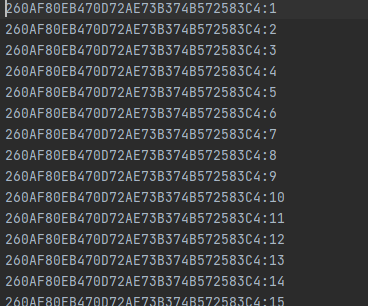
\includegraphics[width=\linewidth]{images/notesetpicture1sm.png}
  \caption{Extract of a generic Note Set file}\label{fig:ns_example_1}
\endminipage\hfill
\minipage{0.49\textwidth}
  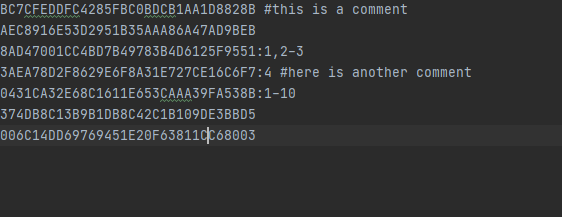
\includegraphics[width=\linewidth]{images/notesetpicture2.png}
  \caption{Extract of a Note Set file using abbreviations and comments}\label{fig:ns_example_2}
\endminipage\hfill
\end{figure}

\subsection{The pynoteset library}
Since there is already a comprehensive Python toolchain for Adaptation Software, it was an obvious choice to implement a library  \emph{pynoteset}-  This small library can generate NoteSet object from ASCII-files or lists of FileIds/NoteIds, and perform the classical set-theory operations on NoteSets. The features of the pynoteset library can be summarized as follows: 
\begin{enumerate}
\item generate NoteSet objects from files
\item export NoteSet objects to ASCII files
\item annotate NoteSet objects and parse string annotations
\item merge NoteSet objects: for two NoteSets $A$ and $B$ generate the NoteSet $A \cup B$.
\item intersect NoteSet objects: for two NoteSets $A$ and $B$ generate the NoteSet $A \cap B$.
\item compare NoteSet objects: for two NoteSets $A$ and $B$ generate the NoteSEt $A\backslash B$ and $B\backslash A$. 
\end{enumerate}

The library consists of three main classes, the NoteSet class, the NoteSetAnnotation class and the NoteSetConverter class. The latter's purpose is to generate NoteSet objects from files and lists of strings, a functionality that was outsourced into a converter class because of a dependency on MDS. See the pynoteset class diagram figure \ref{fig:pynoteset} for reference.\
Furthermore, a converter class NoteSet2Notelistfile has been added to the library \emph{notelistfile}, which allows the conversion of NoteSets to Notelistfile, the standard XML based format currently in use. This functionality is particularly powerful since a majority of the python toolchain already uses the Notelistfile model internally. This converter thus provides an interface for the NoteSet object to be used in other tools.\par
For deployment of this library a Bitbucket CI/CD pipeline is used, which deploys the package to a software repository manager (JFrog Artifactory). Thus registrered Artifactory users can install the pynoteset package like any other using pip.
\begin{figure}
 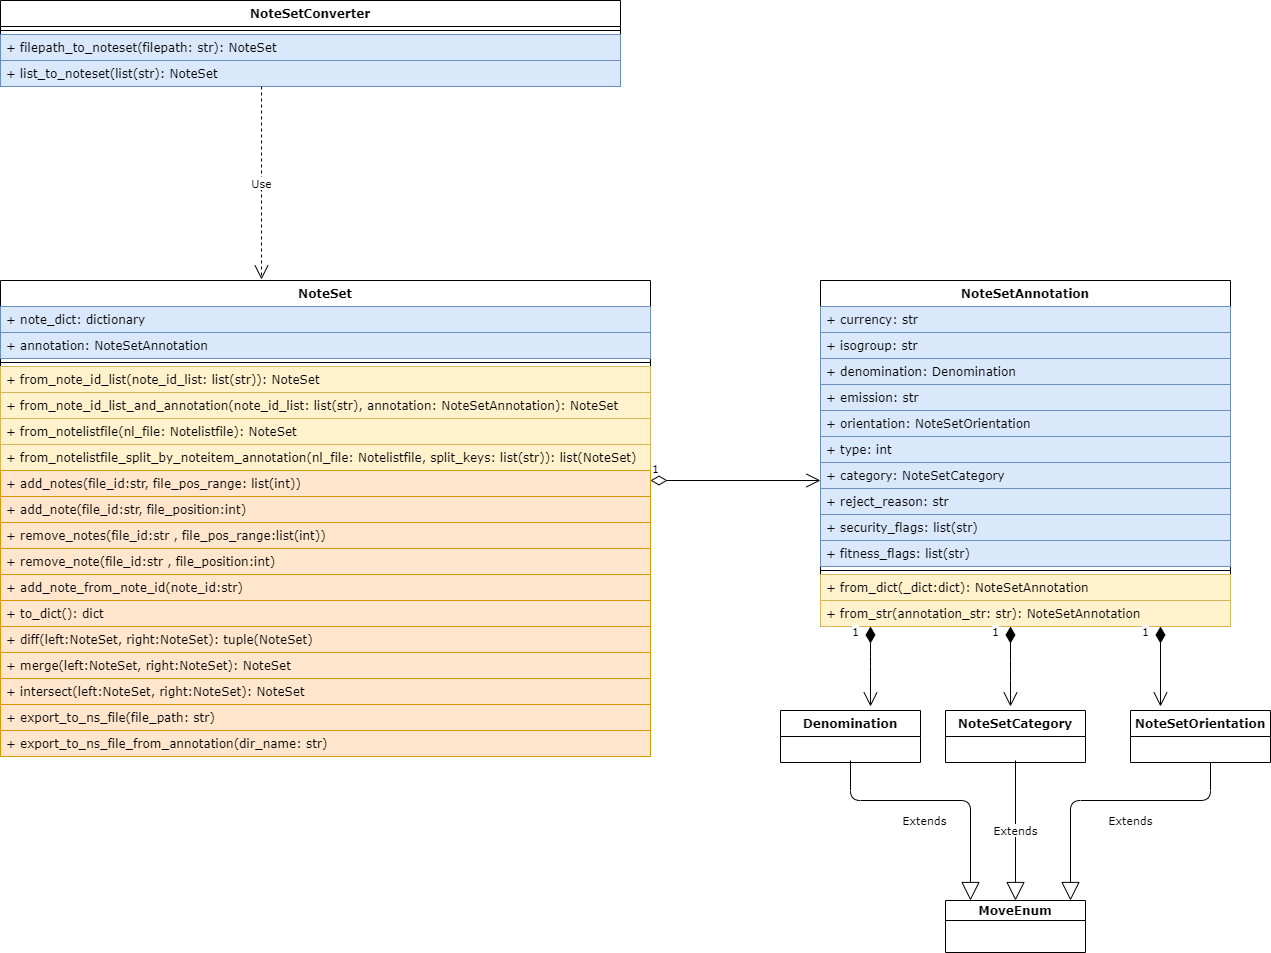
\includegraphics[width=\linewidth]{images/pynoteset.png}
   \caption{Class Diagram of \emph{pynoteset}}\label{fig:pynoteset}
\end{figure}

\section{Note Set Annotation Specification}
\label{ns_annotation_spec}

\subsection{Motivation}
As already mentioned, we introduce Note Sets as a container for notes which are equivalent with respect to a yet to be defined annotation, the labeling of the set. Since the Note Set itself is basically just a set of IDs or keys, all substantial information will be in the annotation. The first challenge is to select the properties which should be part of the annotation. The second is the question of how to persist the annotation within the Note Set. Since we do not want to introduce a new Note container format, it's not possible to add the annotation as a sort of header in an XML or JSON format. This would mean that a new format has been introduced and some kind of schema defined for it. \par
The only option that remains is thus to store the set's annotation within the filename itself when exporting a Note Set to disk. For this a special file format string has to be introduced (see below).
\subsection{Criteria for selecting annotational elements}
The selection of the elements which should be part of the annotation was overall not that easy, on the one hand because there are hundreds of properties in a NIF file and we want to be as specific as possible, on the other hand, a Note Set's annotation should be as simple as possible, namely because we want to persist the annotation in a Note Set's filename, which ideally should be a readable and not too long string.
Finally after having consulted with the adaptation specialist team, the selection was done by the following criteria: The mandatory properties are properties which are needed to identify notes in MCM, the same criteria needed when mapping a loaded note to a reference note in a CDF. The optional properties (with the exception of comment) are criteria for which it is very likely that a user wants to split or filter a set of notes by when analyzing or training algorithms.
\subsection{Mandatory Elements of the Note Set Annotation}
The following attributes form the mandatory part of the Note Set's annotation. These are all derived from properties set in the NOTEMSG2 chunk of the NIF file. 
\begin{description}
  \item[Currency] Corresponds to the ISO string matching the the numeric ISOCODE value in the NOTEMSG2 Chunk.
  \item[IsoGroup] A sub-specification of a currency that is mainly used for the currency GBP (Great Britain Pound), which has different banknotes and issuers for the groups England (BOE), Scotland (SCO), Northern Ireland (IRL), Guernsey (GUE), Jersey (JER) and Isle of Man (MAN). For example, the England GBP would be abbreviated as GBPBOE, the Irish one as GBPIRL.
  \item[Emission] Emission of the notes in the Note Set, corresponds to the value of the Chunk EMISSION in NOTEMSG2
  \item[Orientation] Orientation of the notes in the Note Set, corresponds to to ORIENTATION in NOTEMSG2
\item[Type] NoteType (indicating the reference note this note is matched to by the CDF which was used in recording). For currencies like, GBP with different printers (for example HKD\footnote{Hong Kong Dollar} or GBP\footnote{Great Britain Pound}), this type is necessary to identify a note. For other currencies with only one printer, like CHF, denomination and emission is usually enough to identify a note.
\end{description}

\subsection{Optional Elements of the Note Set Annotation}
The following attributes are optional elements of a Note Set Annotation. They are not identifying properties but qualify a note (set).

\begin{description}
\item[Class] Corresponds to the value CATEGORY in NOTEMSG2 Chunk and is an attribute for authenticity and fitness of a banknote, for example, Category 4a notes are authentic and fit notes, Category 2 are counterfeits. It's a likely use case that a user would want to split notes across a currency by category to train and analyze fitness and security algorithms. 
\item[Security and Fitness flags Flags] Security and Fitness Flags are set by certain algorithms and indicate that a note might be classified as unfit or counterfeit. For example, the fitness flag STAIN indicates that the note has some kind of smudging, the security flag ROBBERY\_INK indicates that the presence of robbery ink was detected. 
\item[Reject Reason] This is an enum value found corresponding to the value REJECT\_REASON in NOTEMSG2 chunk. It indicates the reason why a note was rejected or that it was not rejected.
\item [Comment] This is an optional comment added by the user and the only value which does not come from the NIF file
\end{description}

\subsection{Specifying the file format string}
As already stated, the Note set's annotation is to be converted into a filename when exporting a Note Set to ASCII. The file format string to be constructed has to be readable, complete and indicate the optionality of properties, i.e. distinguish the optional properties from the mandatory ones. Finally, the goal is to codify the format into a regular expression and implement an annotation parser in the python noteset library \emph{pynoteset}.
\subsubsection{Preliminary Decisions}
\begin{itemize}
\item The file format string must be defined in a regular expression. Thus any tool which would later adopt the paradigm of Not Sets could easily validate Note Set annotations independent of the programming language.
\item Generic placeholder for non-specified mandatory properties: Since we allow Note Sets to be merged, we have to anticipate the scenario where e.g. a Note Set contains notes of various denominations. Therefore we need a placeholder for all mandatory properties indicating the state of 'Undefined' or mixed. This placeholder is 'XXX' for currencies and isogroups and 'X' otherwise, a practice which is already in use in the recording of note data and thus one that users are already familiar with. 
\item Allowing of both upper- and lowercase spelling: While it is common to use uppercase notation for currency ISO codes and isogroups and lowercase spelling for emissions, we will allow both upper- and lowercase notation to make the already fairly complicated string format less restrictive.
\end{itemize}
Finally, such a regular expression could be defined as follows:

\begin{center} 
\begin{verbatim}
([A-Z]{3}){1,2}_(([0-9]*[.])?[0-9]|X)*_([a-z]|X)_([1-4]|X)_([1-9]+|X)(_CL[1-4])?(_SF\(([A-Z_0-9]+)(&[A-Z_0-9]+)*\))?(_FF\(([A-Z_0-9]+)(&[A-Z_0-9]+)*\))?(_[a-zA-Z0-9]*)?
\end{verbatim}
\end{center} 
The examples in figure \nameref{fig:ns_example} illustrate the application of this regular expression, i.e. some valid Note Set Annotation file strings
\begin{figure}[!htb]
  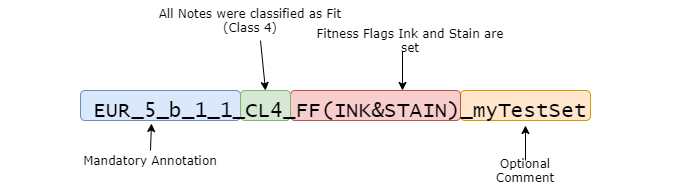
\includegraphics[width=0.49\linewidth]{images/annotation_example1.png}
  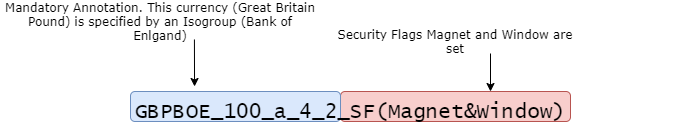
\includegraphics[width=0.49\linewidth]{images/annotation_example2.png}
  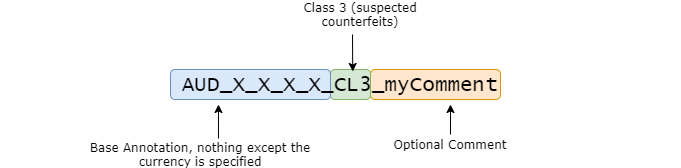
\includegraphics[width=0.49\linewidth]{images/annotation_example3.png}
  \caption{Note Set Annotation Examples}\label{fig:ns_example}
\end{figure}

A parser for annotation strings was included in the pynoteset library and since we have defined a regex for it, it would be relative easy to implement this feature in other tools as well.


